\documentclass[12pt]{article}

\usepackage[utf8]{inputenc}
\usepackage[margin=0.6in]{geometry}

\usepackage{amsmath}
\usepackage{graphicx}
\usepackage{booktabs}

\title{Ph 223 Problem Set 1}
\author{Alex Zahn}
\date{10/7/2016}

\begin{document}

\maketitle

\newcommand{\wmsq}{W/\(\mathrm{m}^2\,\)}
\newcommand{\msq}{\(\mathrm{m}^2\,\)}
\newcommand{\micron}{\(\mu\mathrm{m}\)\,}
\newcommand{\mcb}{\(\mathrm{m}^3\,\)}

\section{Mean Molecular Weights}

\subsection*{a}

I discovered while doing this problem that pandas dataframe objects have a to\_latex() method. The column header alignment comes out a bit off, but it's really impressive for being an intervention-free solution.

\begin{center}
\begin{tabular}{llllrrr}
\toprule
{} &          X &           Y &             Z &   \(\mu\) &  \(\mu_e\) &  \(\mu_i\) \\
\midrule
Anders89   &  0.9096698 &  0.08887474 &   0.001455488 &  0.534063 &   1.055256 &   1.081314 \\
Asplund09  &  0.9206905 &  0.07835076 &  0.0009587071 &  0.530184 &   1.049246 &   1.071727 \\
Feldman92  &   0.909657 &  0.08887349 &   0.001469519 &  0.534068 &   1.055263 &   1.081327 \\
Anders82   &   0.924508 &  0.07405309 &    0.00143894 &  0.528887 &   1.047181 &   1.068582 \\
Grevesse98 &  0.9204288 &  0.07832849 &   0.001242676 &  0.530289 &   1.049388 &   1.072010 \\
Wilms00    &  0.9101783 &  0.08892442 &  0.0008972954 &  0.533854 &   1.054976 &   1.080751 \\
Lodders03  &  0.9257495 &  0.07331936 &  0.0009311188 &  0.528432 &   1.046511 &   1.067425 \\
\bottomrule
\end{tabular}
\end{center}

\subsection*{b}

For a fully ionized, pure carbon star, we should have \(\mu_I \approx 12\), \(\mu_e \approx 1\), and \(\mu = (\mu_I^{-1} + \mu_e^{-1})^{-1} \approx .92\)

So we might expect that, at the same mass, a carbon rich star has a higher density than a hydrogen rich star because it has fewer particles from which an equation of state might generate pressure, and thus that it should have a lower radius.


\section{Spectrophotometric Distance Estimates of Binary Stars}

\subsection*{a}

For Proxima Centauri, we have a parallax angle of 768.13 mas, which corresponds to a distance of about 1.3 pc. Looking at the definition of apparent and absolute magnitude, we can convert between the two using \(m-M = 5\log_{10}{(d/10)}\), for \(d\) in parsecs. This yields \(M_V = 15.6\), \(M_J = 9.8\), \(M_U = 18.6\), and \(M_B = 17.4\)

For the sun, we have \(d = 4.848 \times 10^{-6}\) pc, with  \(M_V = 4.8\), \(M_J = 3.6\), \(M_U = 5.6\), and \(M_B = 5.5\). So the sun is quite a lot brighter in these bands.

\subsection*{b}

Assuming 42 Makeyupus shares the same \(M_J\) as Proxima Centauri, we get that \( 5\log_{10}(d/10) = 12.45-9.785\) for a distance of 34.12 pc.

\subsection*{c}

I interpret the question to mean that previously, we were misattributing observed flux from the secondary to the primary while still guessing the luminosity correctly. So I think we're supposed to take the measured J band flux down by \(1/1.3 \approx .77\), find the resulting \(m_J\), and then estimate a distance based on \(M_J\) from above.

Recall \(m = -2.5\log_{10}(f/f_0)\). If the flux is now \(.77f\),  \(m=-2.5(\log_{10}(f/f_0)) -2.5 \log_{10}.77 \). So \(m_J\) is higher by about .284, and our new distance estimate is 38.9 pc.




\section{HR Diagram}

Below we have an HR diagram generated from the theoretical values from the course website. Black points are dwarf stars, red points are giants, and blue points are supergiants. O type stars are plotted with an open circle. Lines of constant radius are shown for .2, 1, 5, 10, 50, 100, 500 and 2500 solar radii. We can see that (at least of the theoretical stars we're given) most giants are between five and fifty solar radii and most supergiants are between and twenty five hundred solar radii. I will look into annotating the graph with labels for the lines of constant radius eventually.

\begin{center}
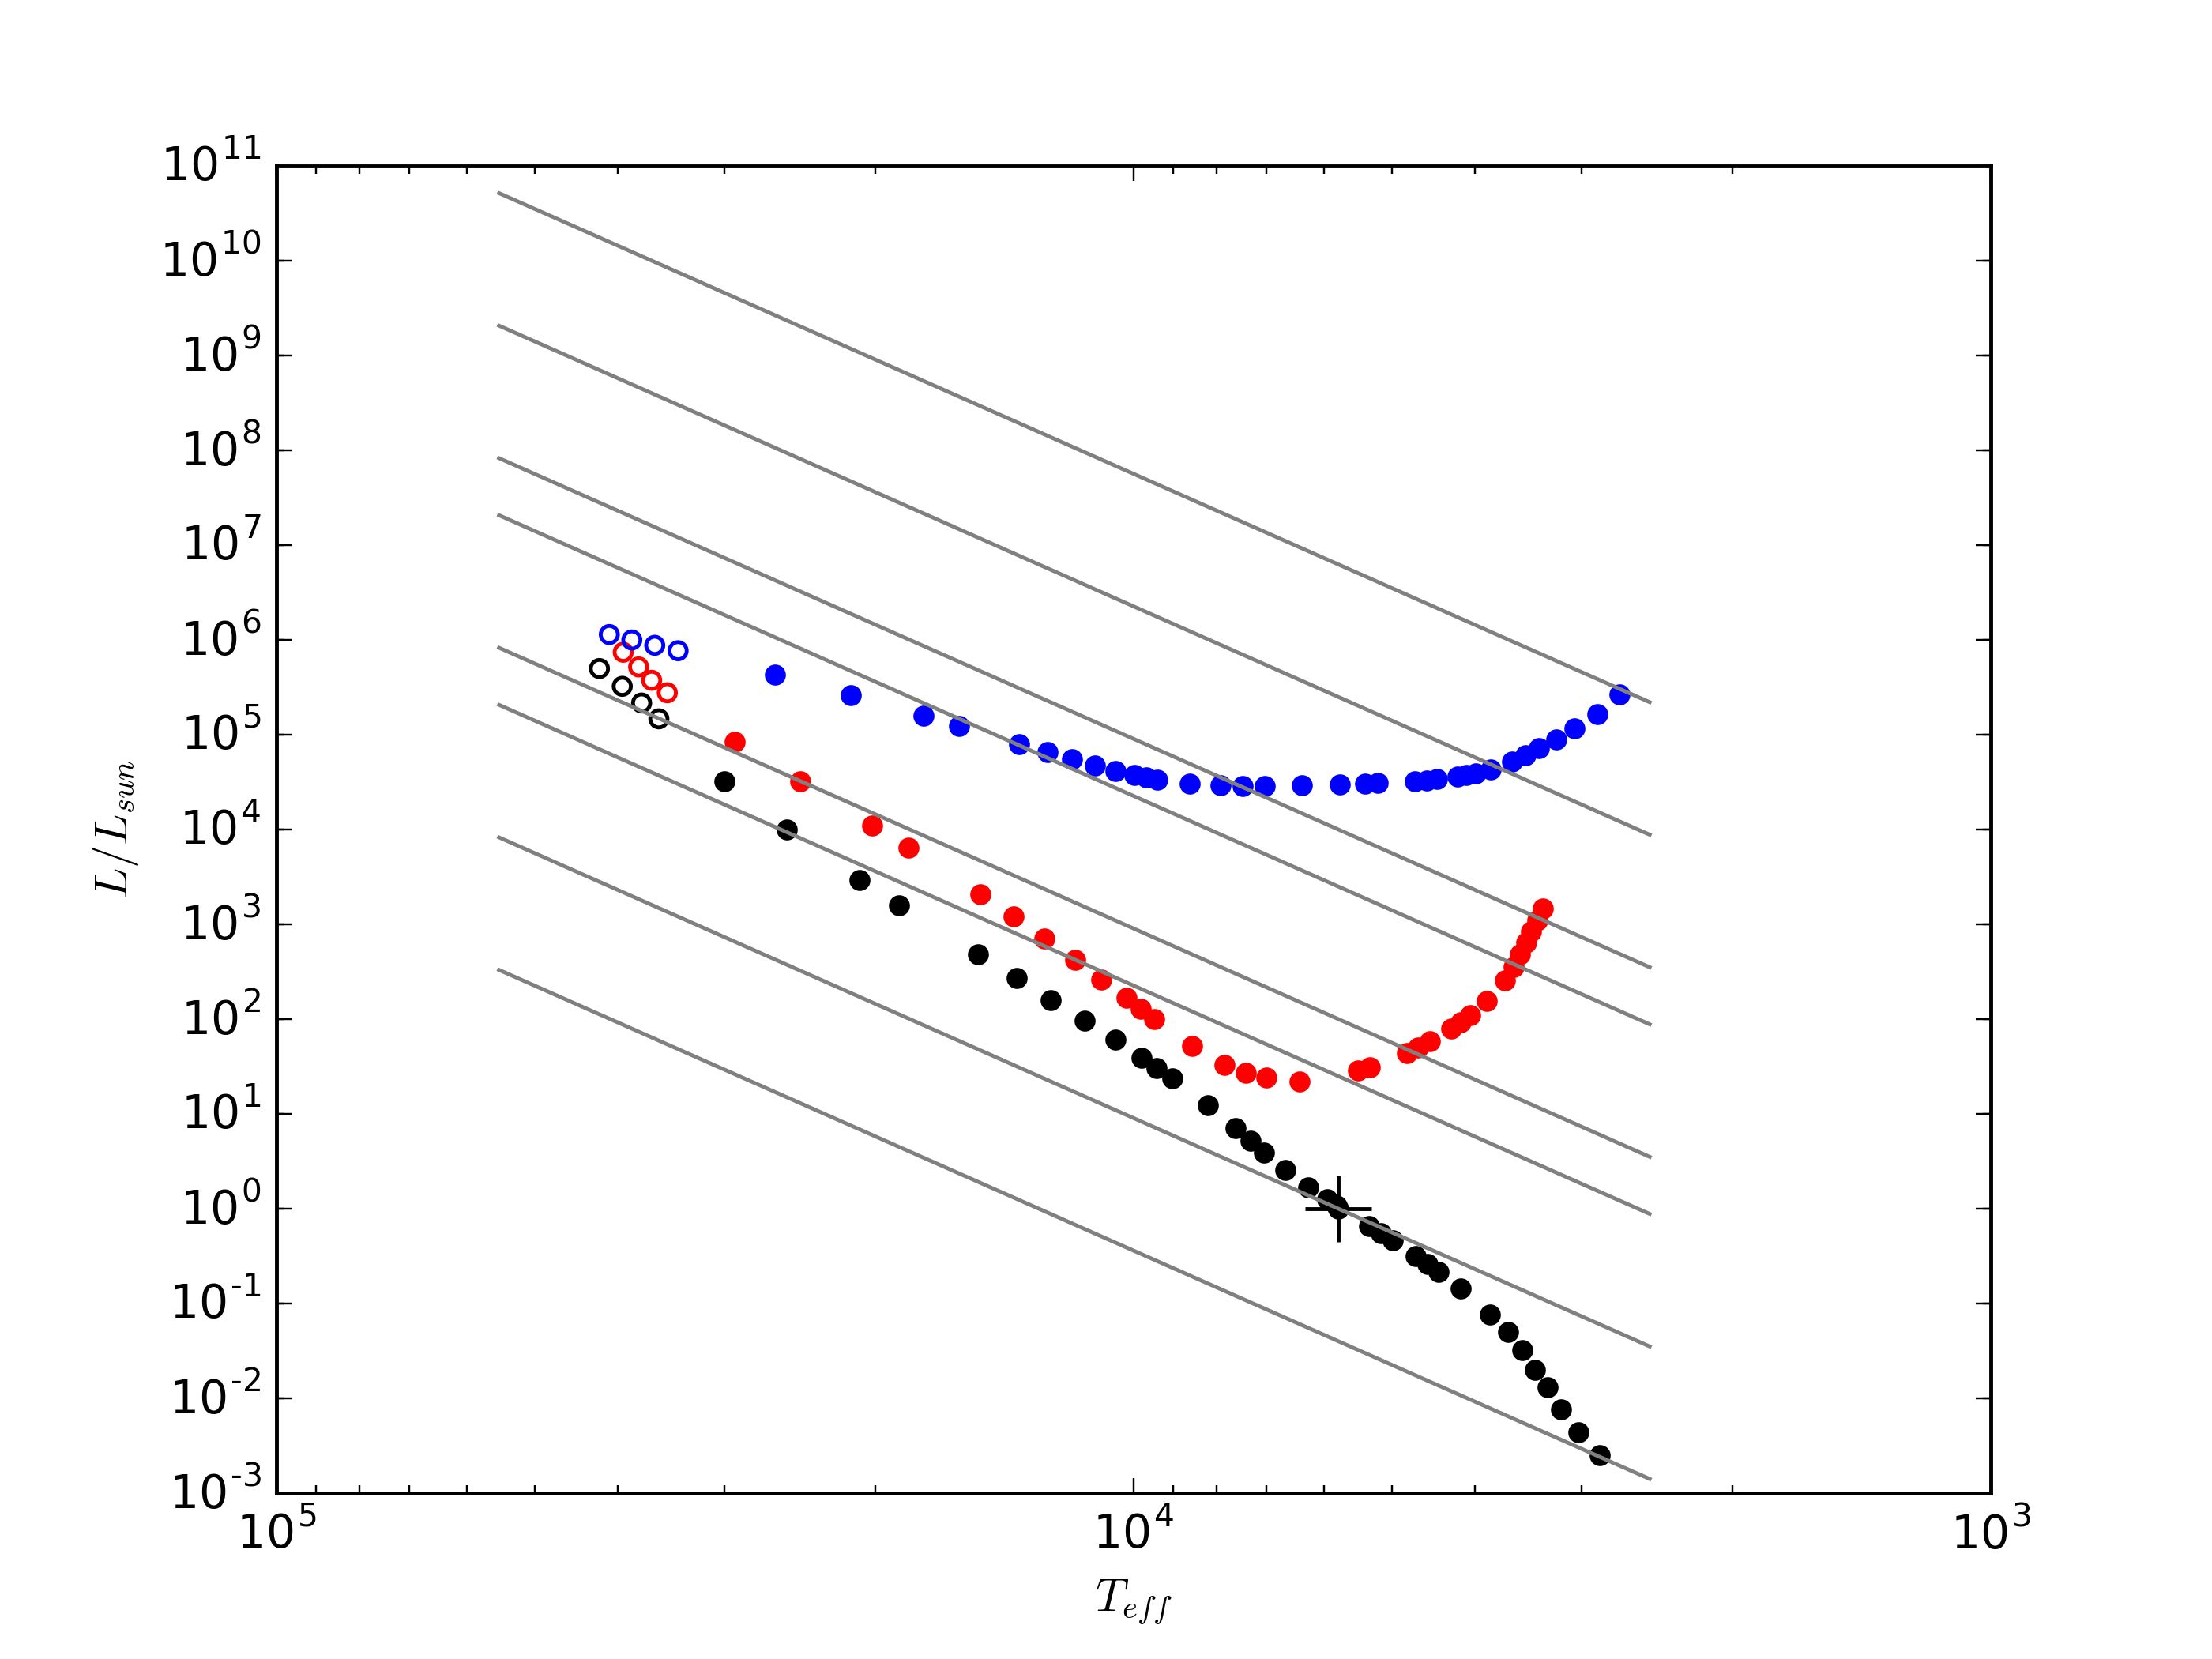
\includegraphics[scale=.7]{HR.png}
\end{center}



\section{A Simple Star Model}

\subsection*{a}

From mass continuity, \(\frac{dr}{dm} = \frac{1}{4\pi r^2 \rho}\). With our assumed density profile, this is a separable equation:

\[ \int 4\pi \rho_c r^2\left(1-\frac{r}{R}\right)dr = \int dm
\]

\(r(m=0) = 0\) so that we have

\[ 4\pi \rho_c \left( \frac{r^3}{3} - \frac{r^4}{4R} \right) = m
\]

From hydrostatic equilibrium, \(\frac{dP}{dr} = \frac{-Gm}{r^2}\rho\). We've just found \(m\) as an explicit function of \(r\), so we can integrate this for the pressure profile right away.

\begin{align*}
P &= P_c + \int_0^r \frac{dP}{dr}dr \\[12pt]
&= P_c - \int_0^r 4\pi\rho_c G \left(  \frac{r}{3} - \frac{r^2}{4R} \right)\left( \frac{1}{r^2} - \frac{1}{Rr} \right)dr \\[12pt]
&= P_c - \frac{1}{36R^2} \pi\rho_c G r^2\left( 9r^2 -28Rr + 24R^2 \right)
\end{align*}

So the surface pressure \( P_s \equiv P(R)\) is \(P_c - \frac{5}{36}\pi\rho_c G R^2\). One hopes that \(P_s \ll P_c\), in which case \(P_c \approx \frac{5}{36}\pi\rho_cG R^2\). From the form we already have for \(m\), \(M = m(R) = \frac{1}{3}\pi\rho_c R^3 \) so that we can write

\[ P_c \approx \frac{5}{4\pi\rho_c}G\frac{M^2}{R^4}
\]

although the dependence isn't really \(M^2/R^4\) since we know \(\rho_c = 3M/\pi R^3\). A better expression is

\[ P_c = \frac{5GM}{12R}\]

\subsection*{b}

Right away we have a solar \(P_c\) of \(8\times 10^{10}\) Pa and \(\rho_c\) of 5600 kg/m\(^3\). \(\rho_c\) comes off as on the low end---only 5.6 times that of water on Earth, but then our density profile isn't especially realistic.

If the core is fully ionized, \(\mu_e \approx 2/(1+X) \approx 1.5\). If the metals have an atomic mass of about 12, we have \(\mu_I \approx ( X + Y/4 + Z/12 )^{-1} \approx .46\). So  \(\mu \approx .35\) and the number density at the core is \(n = \rho_c N_{A}/\mu \approx 9.6 \times 10^{27}\) m\(^{-3}\). In the ideal gas approximation, we get \(T_c = P_c/nk_B \approx 6 \times 10^5\) K, which is understandably low given we've underestimated the core density.




\section{MESA}

Looks like MESA is running on my lab machine, and that the tutorial runs evolve the star to sixty thousand and and ten million years:

\begin{center}
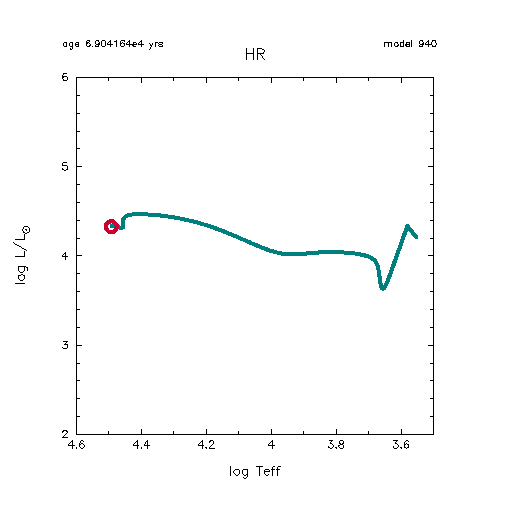
\includegraphics[scale=.7]{HR_pre.png}
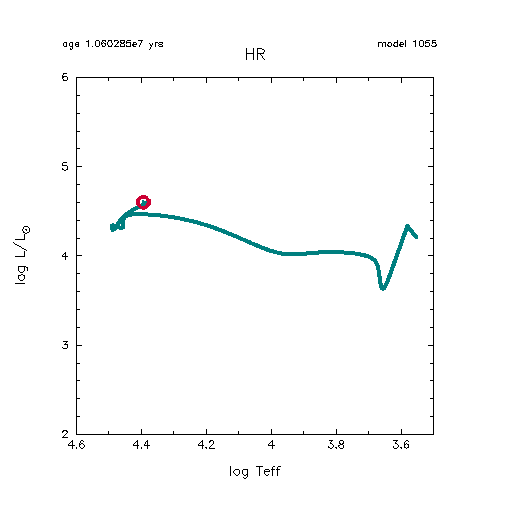
\includegraphics[scale=.7]{HR_post.png}
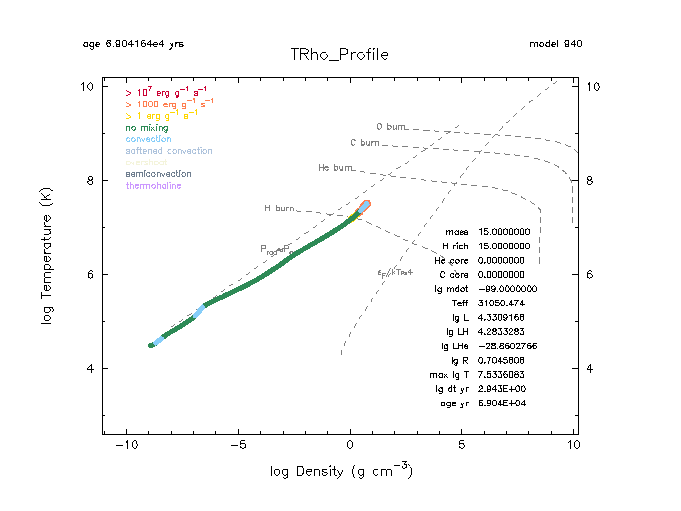
\includegraphics[scale=.6]{trho_pre.png}
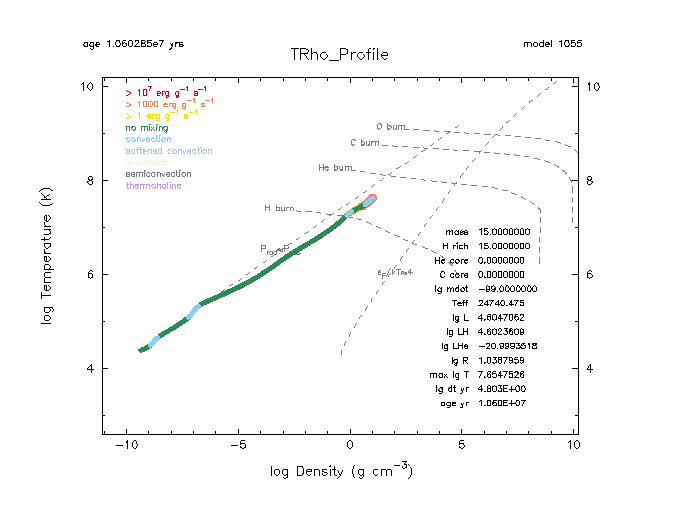
\includegraphics[scale=.6]{trho_post.png}
\end{center}



\end{document}